\documentclass[12pt]{article}
\usepackage[margin=1in]{geometry} 
\usepackage{amsmath}
\usepackage{amssymb}
\usepackage{amsthm}
\usepackage{accents}
\usepackage{graphicx}
\usepackage[dvipsnames]{xcolor}

\setlength{\oddsidemargin}{0in}
\setlength{\textwidth}{6.5in}
\setlength{\topmargin}{-.55in}
\setlength{\textheight}{9in}
\pagestyle{empty}

\begin{document}
\noindent Math 5510

\noindent Topology

\noindent Stephanie Klumpe

\vspace{.2in}
\begin{center}
Problem Set 5
\end{center}


\begin{enumerate}
\item (\#3 in 4.2) Show that $\mathcal{B}_s$ is a basis for a topology on $\mathbb{R}^2$. Specifically, show that $\mathcal{B}_s$ satisfies conditions (1) and (2) of Definition 4.2.1 on page 74 of the text.

When proving that condition (2) holds, you may support your argument with diagrams. However, you must be sure that your diagrams cover all possible cases, are clearly drawn and accompanied by an explanation.\\\\
Let $\mathcal{B}_s$ be as given in class and in the text. Consider any point $(x,y)\in\mathbb{R}^2$. Then take $S_{\epsilon}((x,y))$, the square centered at $(x,y)$, for any $\epsilon>0$. Then $(x,y)\in S_{\epsilon}((x,y))$. Since $(x,y)$ was arbitrary, we have that $\bigcup_{B\in\mathcal{B}_s}B=\mathbb{R}^2$ and $\mathcal{B}_s$ covers $\mathbb{R}^2$. Now, fix $(x_1,y_1), (x_2,y_2)\in\mathbb{R}^2$ and let $S_{\epsilon_1}((x_1,y_1)), S_{\epsilon_2}((x_2,y_2))\in\mathcal{B}_s$ be such that $S_{\epsilon_1}\cap S_{\epsilon_2}\neq\emptyset$, and let $(x,y)\in S_{\epsilon_1}\cap S_{\epsilon_2}$. Now take $\epsilon_3=min\{\epsilon_1-max\{|x-x_1|,|y-y_1|\}, \epsilon_2-max\{|x-x_2|, |y-y_2|\}\}$. Also take $(x_3,y_3)\in\mathbb{R}^2$ where $$x_3=\frac{max\{|x-x_1|<\epsilon_1, |x-x_2|<\epsilon_2\}+min\{|x-x_1|<\epsilon_1, |x-x_2|<\epsilon_2\}}{2}$$and $$y_3=\frac{max\{|y-y_1|<\epsilon_1, |y-y_2|<\epsilon_2\}+min\{|y-y_1|<\epsilon_1, |y-y_2|<\epsilon_2\}}{2}$$That is, we are setting $(x_3,y_3)$ to be the midpoint of the intersection of $S_1$ and $S_2$. Then $S_{\epsilon_3}((x_3,y_3))\in\mathcal{B}_s$ such that $(x,y)\in S_{\epsilon_3}((x_3,y_3))\subseteq S_{\epsilon_1}((x_1,y_1))\cap S_{\epsilon_2}((x_2,y_2))$ as shown in the diagram below. Here we show squares to be in the first quadrent for simplicity, but since the centers of $S_1$ and $S_2$ are arbitrary, this need not be the case. So, by the diagram, we see that when the intersection of 2 squares is non empty, there exists a square with length $\frac{\epsilon}{2}$ that is a subset of the intersection that contains the arbitrary point $(x,y)$. Thus, we have that $B_s$ is a basis for some topology on $\mathbb{R}^2$.
\begin{center}
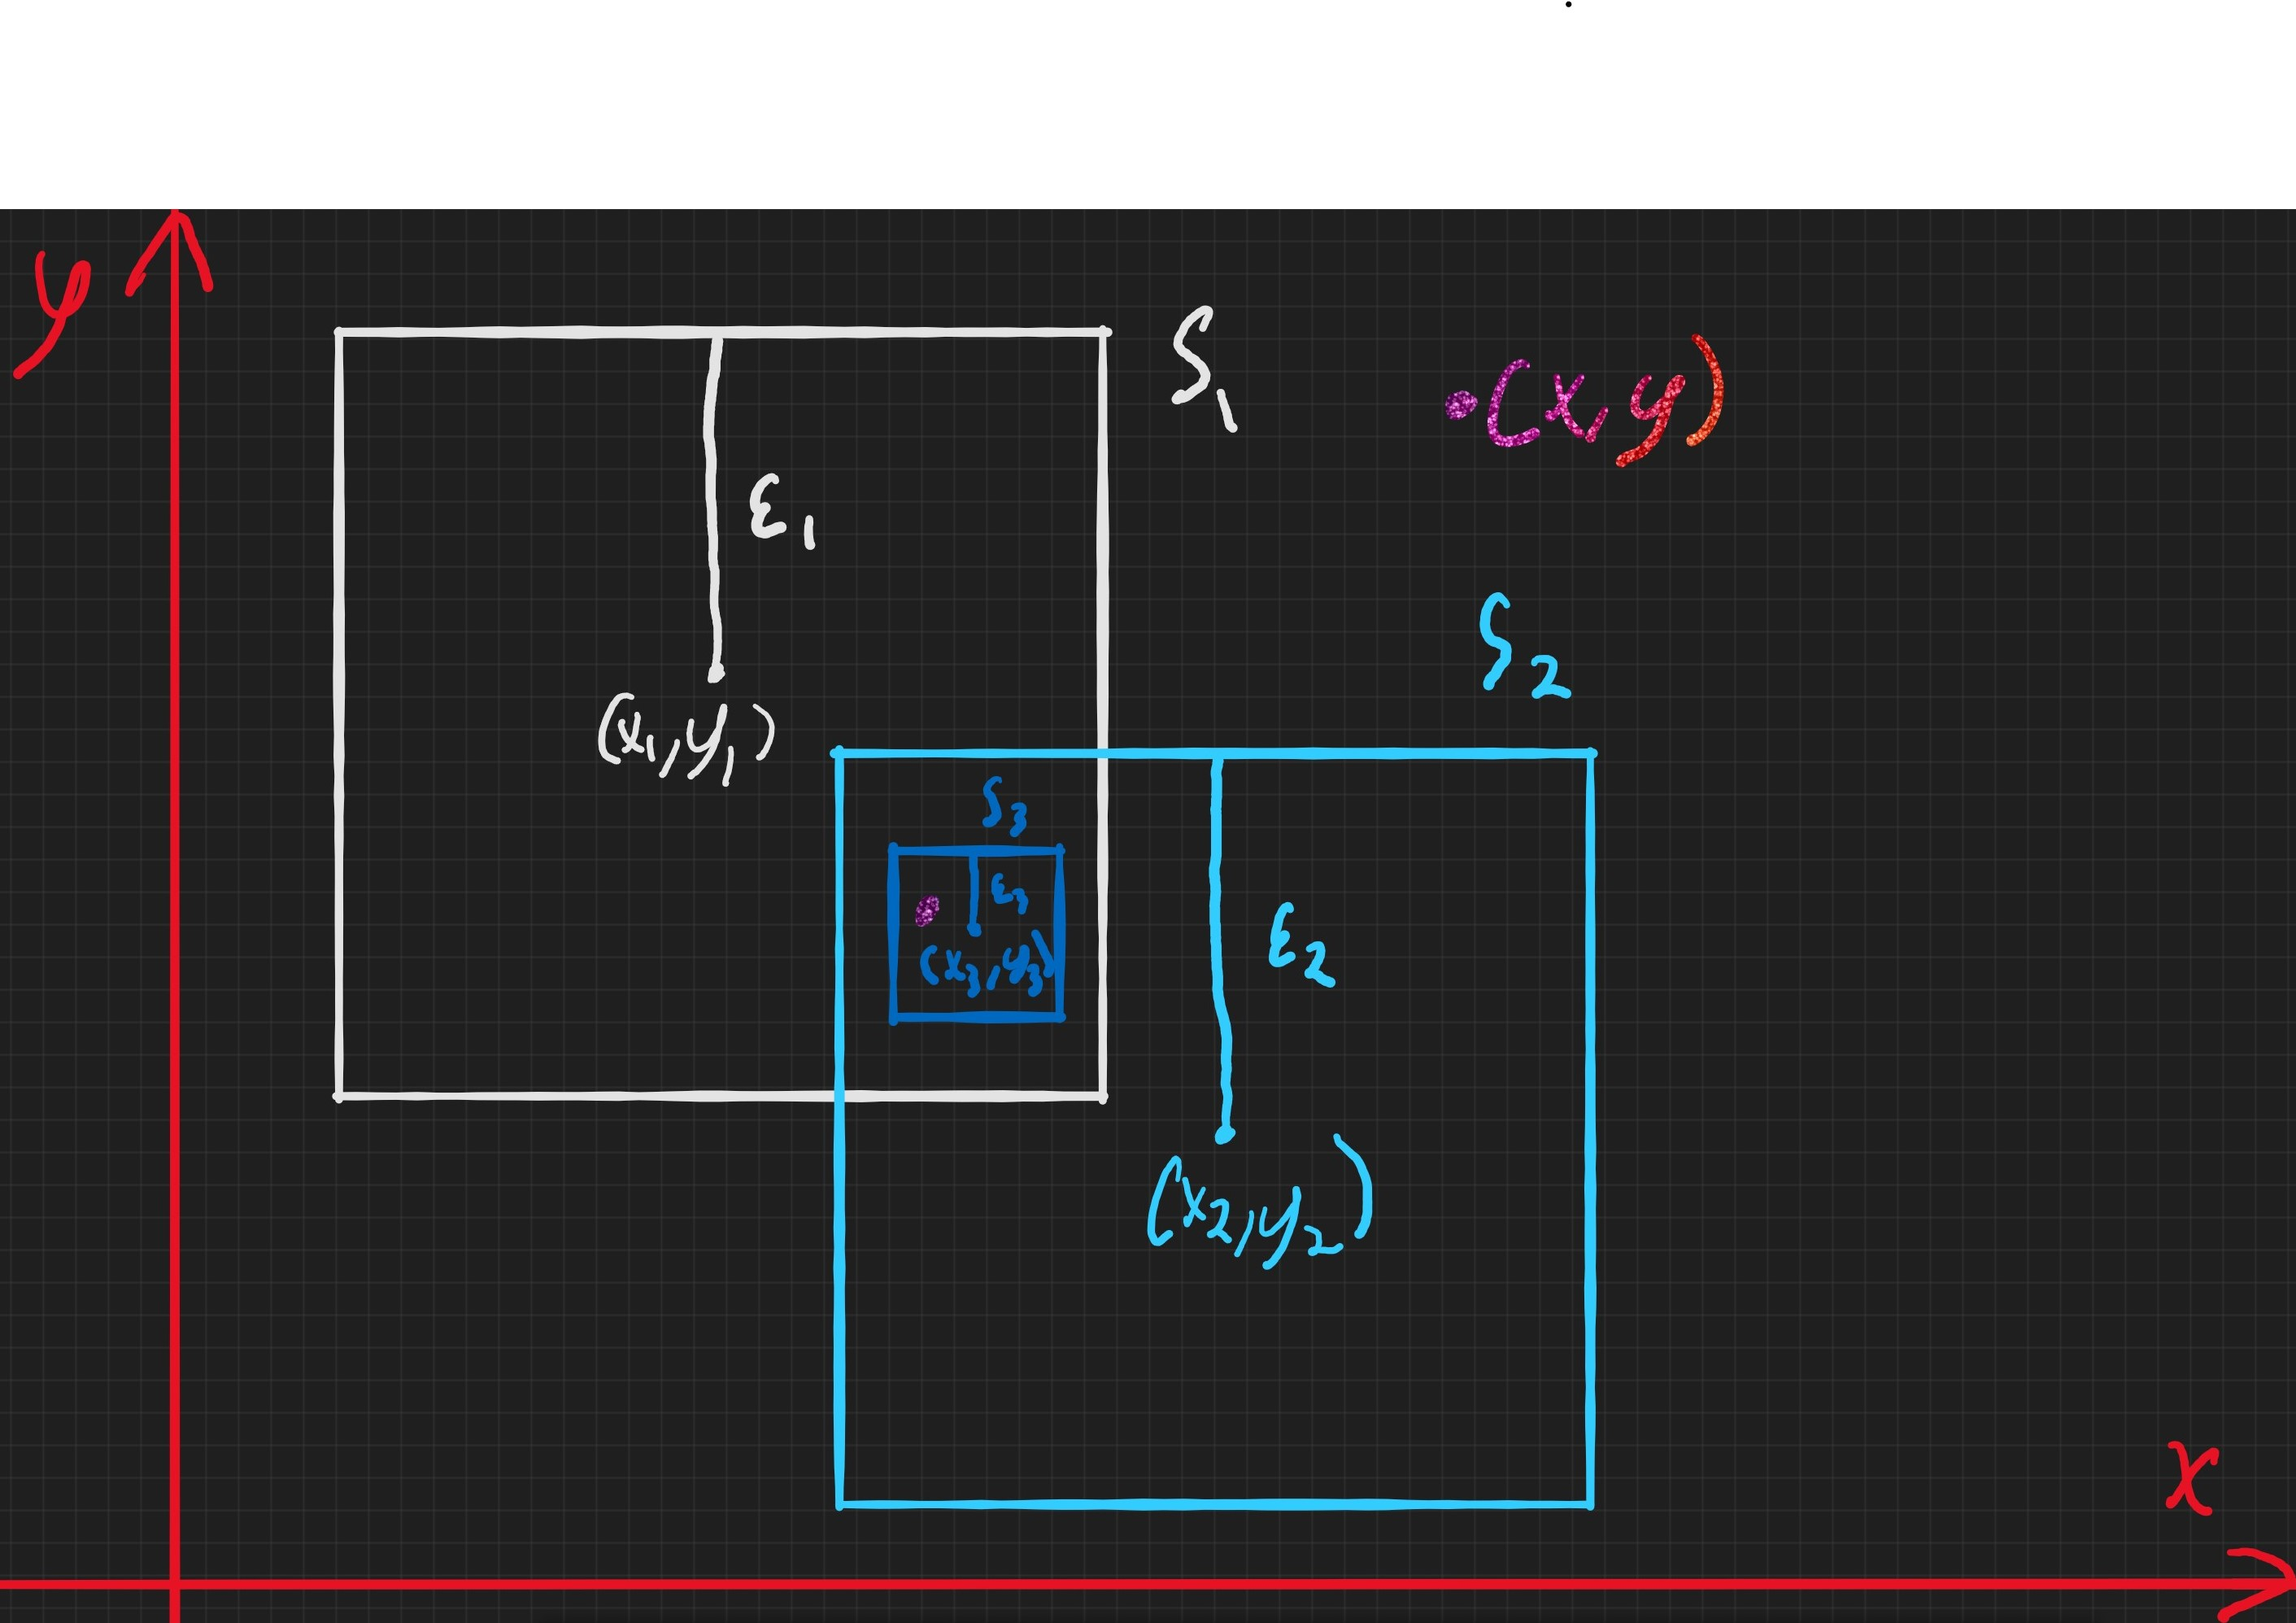
\includegraphics[scale=0.37]{ps5p1.JPG}
\end{center}

\item (\#2 in 4.2) Show that for $\mathcal{B} = \{(r_1,r_2)| r_1,r_2 \in \mathbb{Q}, r_1 < r_2\}$, we have $\tau_{\mathcal{B}} = \mathcal{U}$, the usual topology on $\mathbb{R}$. (In order to show that two topologies are equal, use double containment).\\\\
Let $\mathcal{B}$ and $\mathcal{U}$ be as given. Now, $\tau_{\mathcal{B}}=\{U\subseteq\mathbb{R}|$ if $x\in U$ then there exists $B\in\mathcal{B}$ such that $x\in B\subseteq U\}$. First, let $X\in\tau_{\mathcal{B}}$. If $X=\emptyset$ or $X=\mathbb{R}$, then $X\in \mathcal{U}$. So, let $X$ be a proper nonempty subset of $\mathbb{R}$. So $X$ is such that if $x\in X$, then there exists $(r_1,r_2)\in\mathcal{B}$ for some $r_1<r_2\in\mathbb{Q}$ such that $x\in(r_1,r_2)\subseteq X$. So, $X\in\mathcal{U}$ by definition of the usual topology. Now, let $X\in\mathcal{U}$. If $X=\emptyset$ or $X=\mathbb{R}$, then $X\in\tau_{\mathcal{B}}$. So, let $X\subset\mathbb{R}$ be such that $X\neq\emptyset$. So, by definition, if $x\in X$ then there exists $(a,b)$ for some $a<b\in\mathbb{R}$ such that $x\in(a,b)\subseteq X$. Now, by the density of the rationals, there exist $r_1,r_2\in\mathbb{Q}$ such that $a\leq r_1<x<r_2\leq b$. So, there exists $(r_1,r_2)$ for some $r_1,r_2\in\mathbb{Q}$ with $r_1<r_2$ and such that $x\in(r_1,r_2)\subseteq X$. Therefore, $X\in\tau_{\mathcal{B}}$. Thus, $\tau_{\mathcal{B}} = \mathcal{U}$ as desired.

\item Let 

$\begin{array}{rcl}
\mathcal{B}_1&=&\{(a,b)|a < b\}\\
\mathcal{B}_2&=&\{(a,+\infty)|a\in \mathbb{R}\}\\
\mathcal{B}_3&=&\{(-\infty,b)|b\in\mathbb{R}\}
\end{array}$

be collections of subsets of $\mathbb{R}$. Assuming that each of these is the basis of some topology on $\mathbb{R}$, show that $\mathcal{B}_2\cup \mathcal{B}_3$ is a sub-basis for the topology generated by $\mathcal{B}_1$.\\\\
Let $\mathcal{B}_1, \mathcal{B}_2,$ and $\mathcal{B}_3$ be as given. Now, fix $b_0\in\mathbb{R}$, and take $a_0\in\mathbb{R}$ such that $a_0<b_0$. Now clearly, $(a_0,\infty)\in\mathcal{B}_2$ and $(-\infty,b_0)\in\mathcal{B}_3$, and so $(-\infty,b_0)\cup(a_0,\infty)=\mathbb{R}$. Hence, $\bigcup(\mathcal{B}_2\cup\mathcal{B}_3)$ covers $\mathbb{R}$. Now let $\mathcal{I}\in\mathcal{B}_1$. Then $\mathcal{I}=(a,b)$ for some $a,b\in\mathbb{R}$ such that $a<b$. Then, we can see that $\mathcal{I}=(-\infty, b)\cap(a,\infty)$ where $(-\infty, b),(a,\infty)\in\mathcal{B}_2\cup \mathcal{B}_3$. Since $\mathcal{I}$ was arbitrary, we have that every element in $\mathcal{B}_1$ is the intersection of some elements in $\mathcal{B}_2\cup \mathcal{B}_3$. Thus, $\mathcal{B}_2\cup \mathcal{B}_3$ is a sub-basis for the topology generated by $\mathcal{B}_1$.

\item (\#7 in 4.3) Prove that if $A$ is any subset of the indiscrete space $X_{\mathcal{I}}$, with $\text{Card($A$)}\geq 2$, then $A' = X$.\\\\
Let $A\subseteq X_{\mathcal{I}}$ with Card$(A)\geq2$. We have that $A'\subseteq X$ by definition. So, let $x\in X$. Since $\mathcal{I}=\{X,\emptyset\}$, every neighborhood of $x$ is $X$ itself. Since $A\subseteq X_{\mathcal{I}}$ with Card$(A)\geq2$, $(X\setminus\{x\})\cap A\neq\emptyset$. Therefore $x\in A'$. Thus, $X=A'$.

\item If $p$ is an isolated point of a subset $A$ in a topological space $X_{\tau}$, show that there exists a $\tau$-open set $U$ such that $U\cap A = \{p\}$.\\\\
Let $X_{\tau}$ be a topological space and let $A\subseteq X_{\tau}$ with $p$ an isolated point of $A$. By definition, $p\notin A'$. Then $p\notin\{x|$for all neighborhoods $N_x$ of $x, (N_x\setminus\{x\})\cap A\neq\emptyset\}$. That is, there exists a neighborhood, $N_p$, of $p$ such that $(N_p\setminus\{p\})\cap A=\emptyset$. By definition of neighborhood, $N_p$ is $\tau-$open. Thus, there exists a $\tau-$open set, $N_p$, such that $N_p\cap A=\{p\}$ as desired.

\item  Let $X_{\tau}$ be a topological space, and let $A$ and $B$ be subsets of $X$ with $X=A\cup B$. Let $W$ be a subset of $A\cap B$ that is both $\tau_A$-open and $\tau_B$-open. Prove that $W$ is also $\tau$-open. (Hint: Show that $W$ is the intersection of two $\tau$-open sets $V_1$ and $V_2$).\\\\
Let $A, B,$ and $X_{\tau}$ be as given above. Let $X=A\cup B$ and $W\subseteq A\cap B$ be such that $W$ is $\tau_A$ and $\tau_B$-open. If $W=\emptyset$, then $W$ is $\tau-$open. Now assume that $W\neq\emptyset$. Since $W$ is $\tau_A-$open, $W=A\cap V_1$ such that $V_1$ is $\tau-$open. Since $W$ is $\tau_B$-open, $W=B\cap V_2$ such that $V_2$ is $\tau$-open. Now, $W\cap V_1=B\cap(V_1\cap V_2)$ and $W\cap V_2=A\cap(V_1\cap V_2)$. Since $W\subseteq A\cap B$ and by these two equalities, we have that $W=A\cap(V_1\cap V_2)=B\cap(V_1\cap V_2)$. Now, $W=W\cup W=(A\cap(V_1\cap V_2))\cup (B\cap(V_1\cap V_2))=(A\cup B)\cap(V_1\cap V_2)$. Since $X=A\cup B$, we have that $W=X\cap(V_1\cap V_2)=V_1\cap V_2$. Since $V_1$ and $V_2$ are both $\tau$-open, we have that $W$ is also $\tau$-open as desired.

\end{enumerate}


\vspace{.2in}
\noindent Suggested: look at \#1 \& \#3 in 4.3 

\end{document}
